%!TEX root = ../thesis.tex
%*******************************************************************************
%****************************** Fourth Chapter **********************************
%*******************************************************************************
%Here you make the strongest statement concerning observations. Highlight the information you want readers to remember. Explain how the results correlate with the problems you have indicated in the introduction. Describe all new things that are significant in finding a solution.

%The recommendations part is for giving advice and indicating other actions that will help to solve particular problems. Sound your own opinion about the direction of future research. Most of the time you have to write it. Just like a research proposal.

%Acknowledgments part is a paragraph where you mention everyone who helped you with composition. Place all cited and used information resources into one list or form an annotated bibliography if needed.
\chapter{Implementation And Performance Evaluation}


In this section, the implementation and performance evaluation of the edge-to-clound system with proposed method is presented. Furthermore, the information of video datasets and the scenario setup are provided. In this implementation, VA server executes the application of intrusion detection. Although the evaluated platform integrates specific application, it is a general design and can be extended for other application with few modifications. The workflow of the evaluated platform is represented in Figure \ref{fig:sysdesign}. It has two main components:
\begin{itemize}
\item Edge node implementation: The streaming data from camera sources are parsed and the proposed method is applied to detect moving objects in the current frame. If the encoded frame includes the motion, it will be forwarded to a cloud node using its own real-time streaming protocol (RTSP) server. To avoid decoding inaccuracies at the cloud node, all frames from starting time to ending time of the motion are continuously delivered in a connection session. Each session will start with an intra-coded frame.
\item Cloud node implementation: Receiving the forwarded encoded frame with the motion from the edge node over the network and then decoding and placing the output images into the intrusion detection module, which uses YOLO to detect humans.
\end{itemize} 
\begin{figure*}
\centering
 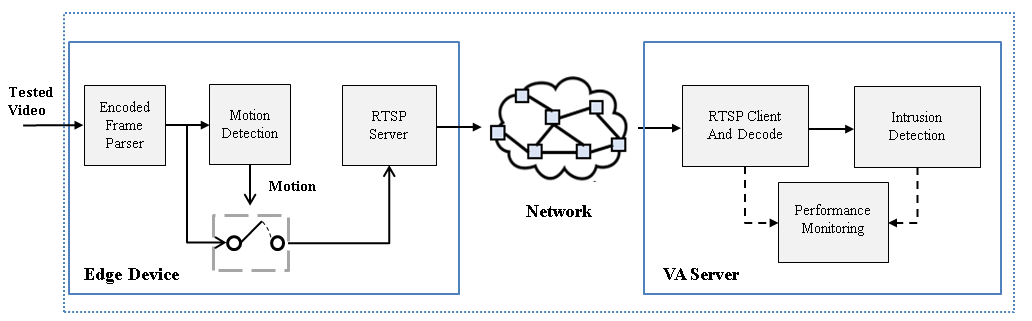
\includegraphics[width=1.1\linewidth]{Figures/SysDesign.png}
 \caption{Overview of System Design}
 \label{fig:sysdesign}
\end{figure*}
\subsection{Scenario Setup}
\begin{figure*}
 \centering
 \subfloat[]
{
  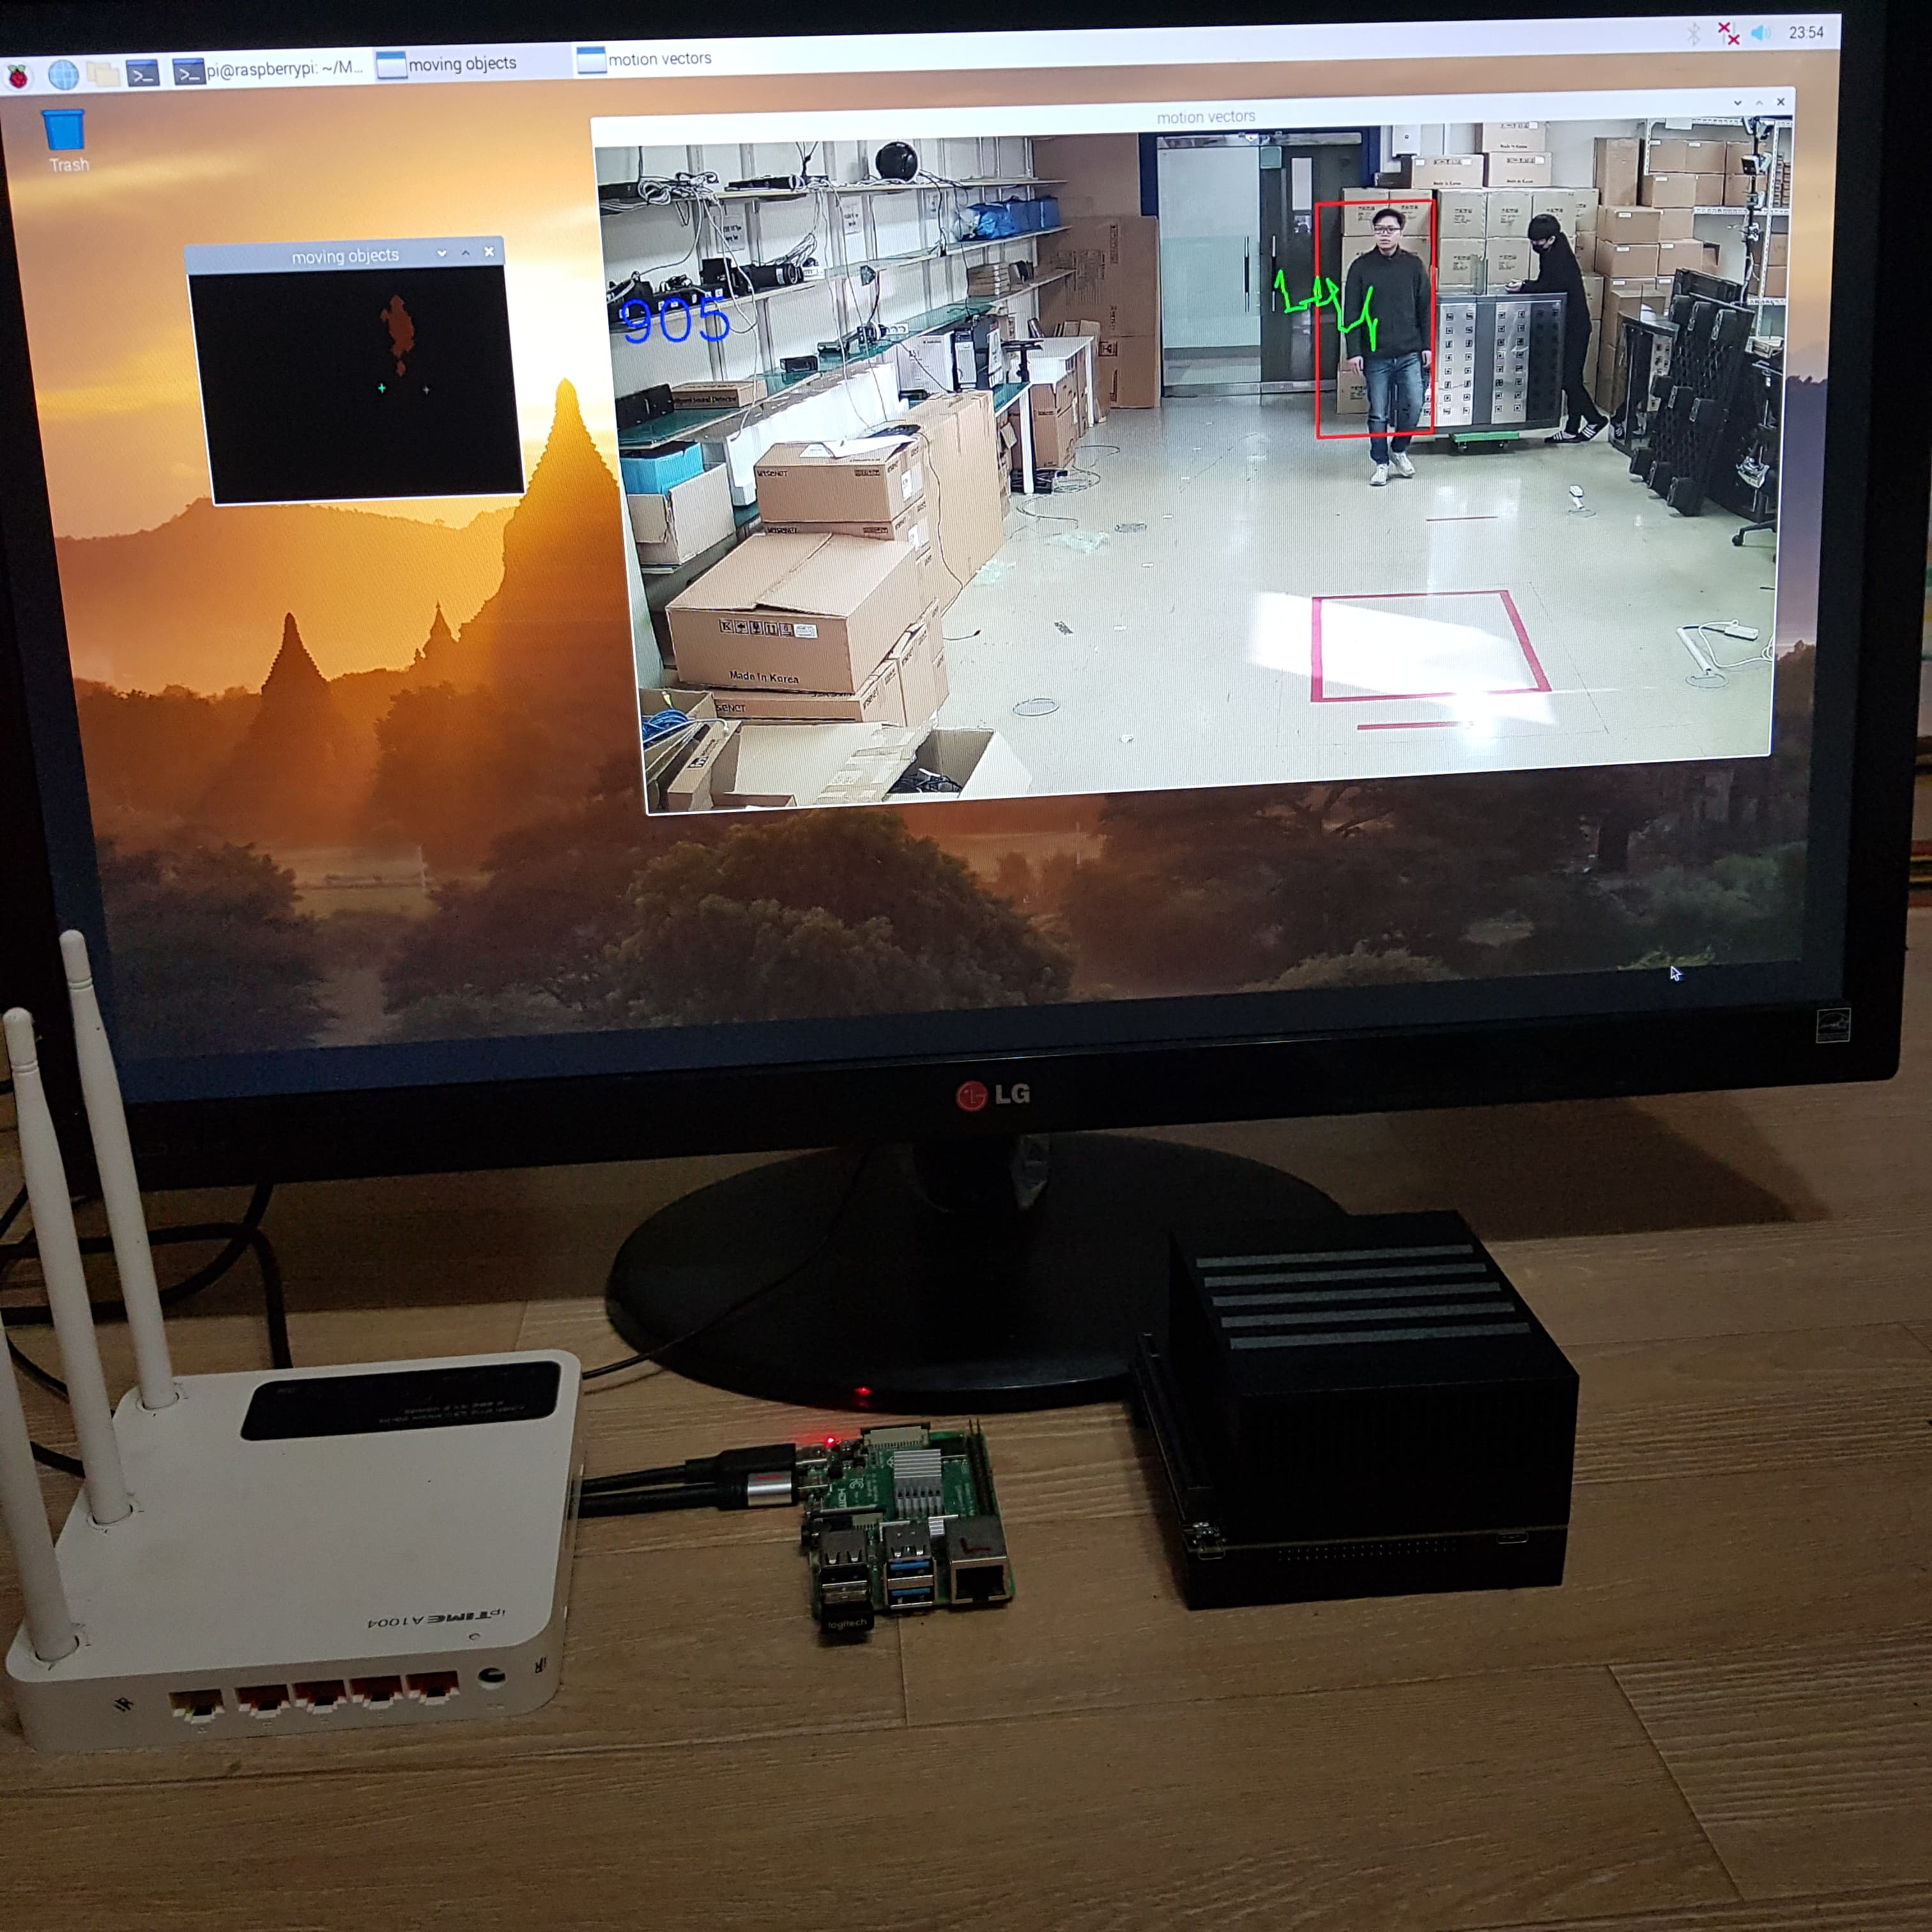
\includegraphics[width=0.5\linewidth]{Figures/TESTBED.jpg}
}
 \subfloat[]
{
  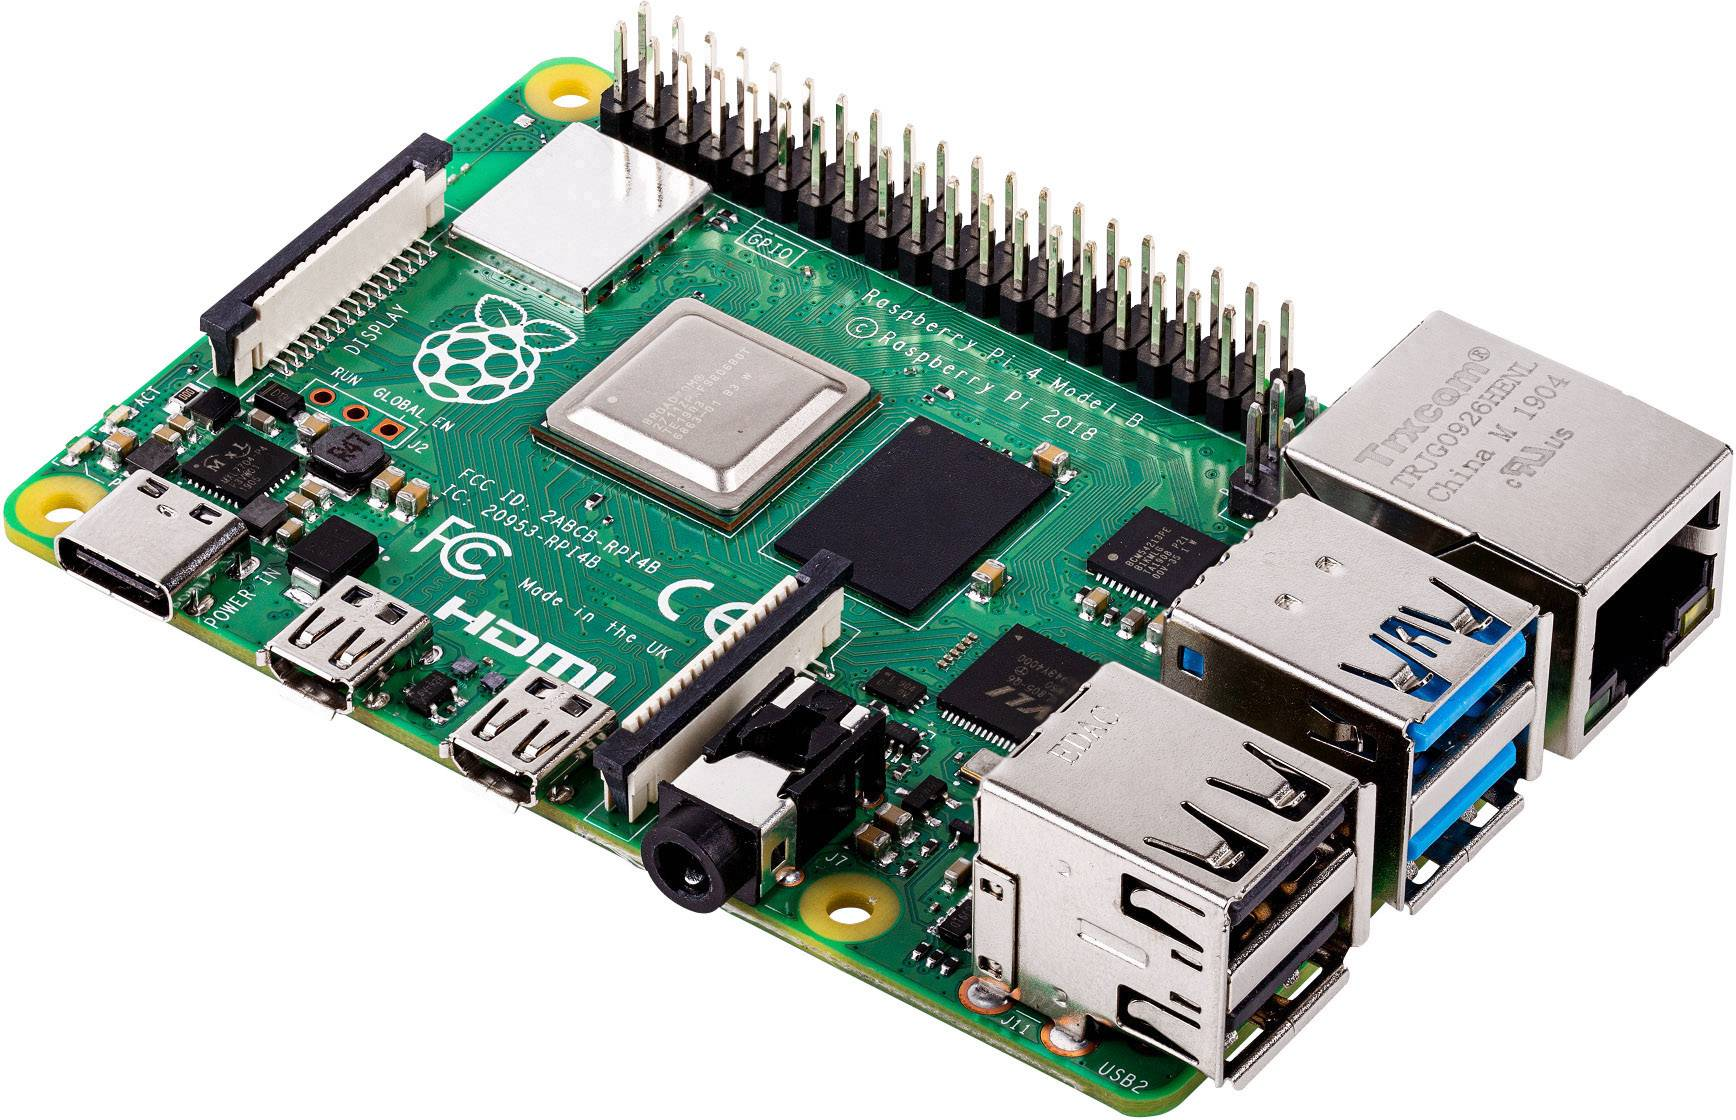
\includegraphics[scale=0.1]{Figures/pi.jpg}
}
  \caption{Testbed: (a) Scenario Setup, (b) The implemendted edge device.}
  \label{fig:testbed}
\end{figure*}
\begin{table}[]
\centering
\caption{Hardware Specifications.}
\label{tab:hw}
\begin{tabular}{|c|c|c|}
\hline
\textbf{Specifications} & \textbf{Edge Device}   & \textbf{Video Analytics Server}                        \\ \hline
Device Name             & Raspberry Pi 4 & NVIDIA Jetson Xavier                                     \\ \hline
Operating System        & Ubuntu 18.04, 64 bits  & Ubuntu 18.04, 64 bits                                  \\ \hline
GPU                     & Not Supported          & NVIDIA Maxwell architecture with  NVIDIA CUDA cores \\ \hline
CPU                     & Quad-core ARM Cortext-A72          & Quad-core ARM Cortext-A57 MPCore processor             \\ \hline
RAM                     & 4 GB                   & 8 GB                                                   \\ \hline
\end{tabular}
\end{table}
\begin{table}[]
\centering
\caption{Video Test Squence.}
\label{tab:videotest}
\begin{tabular}{|c|c|}
\hline
\multicolumn{2}{|c|}{\textbf{Tested Video Information}} \\ \hline
Resolution                        & 1920x1080           \\ \hline
Length                            & 6 minutes           \\ \hline
Codec                             & H264                \\ \hline
Group Of Picture (GOP)            & 30                  \\ \hline
Frame Rate                        & 25                  \\ \hline
\end{tabular}
\end{table}
\begin{table}[]
\centering
\caption{Testbed: Tested Video Grouth-truth motion time.}
\label{tab:motiontime}
\begin{tabular}{|c|c|}
\hline
\textbf{Time}       & \textbf{Duration (Seconds)} \\ \hline
00:00:50 $~$ 00:01:10 & 20                          \\ \hline
00:01:25 $~$ 00:01:45 & 20                          \\ \hline
00:02:12 $~$ 00:01:10 & 5                           \\ \hline
00:02:39 $~$ 00:02:45 & 6                           \\ \hline
00:03:50 $~$ 00:04:48 & 58                          \\ \hline
00:05:00 $~$ 00:05:35 & 35                          \\ \hline
00:05:40 $~$ 00:06:00 & 20                          \\ \hline
Total               & 164                         \\ \hline
\end{tabular}
\end{table}
\begin{itemize}
\item Testbed: We built a testbed comprising a single edge device node and a single video analytics server that runs as a cloud node, as shown in Figure \ref{fig:testbed}. The edge device node involves the moving objects detection and runs on a low-computation device named \textit{Raspberry Pi 4} and video analytics server is executed on \textit{Nvidia- Jetson Xavier} because of a GPU that is supported to run YOLO. The hardware specifications of edge node and video analytics server are then listed in Table \ref{tab:hw}. Note that the two devices are directly connected to a router using a wired cable.
\item Video Test Sequence: experiments have been conducted on the two video datasets. The VIRAT video dataset \cite{VIRAT} was collected in natural scenes showing people performing normal actions for video surveillance domains. The second dataset is previously recorded from the our surveillance camera and uploaded \cite{testvideo}. The details of our video test sequence and the ground-truth motion time are listed in Tables \ref{tab:motiontime} and \ref{tab:videotest}. 
\end{itemize}
We evaluate the performance of the moving object detection method and the proposed edge-to-cloud system separately.

\section{The Light-weight Runtime Moving Object Detection in Video Compressed Domain}
To evaluate the quality of the proposed method for the moving object detection, we calculated the IoU score mettric of the detected object's bounding box with those of the ground-truth bounding box. Because the accuracy of the peoposed method is depend on the MV's density, we run the proposed method multiple times with different scenario application such as: different camera distances, different moving object speeds. We observe that except the I-Frame which does not apply motion estimation, the moving objects including sometimes big MV noises always be detected in other frames. Example of the moving object detection results  are shown in Figure \ref{fig:objectdetect}. 
\begin{figure*}
\centering
\subfloat[]
{
    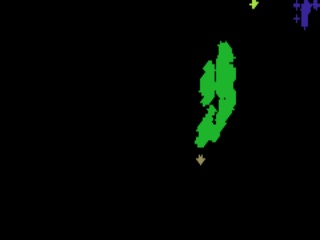
\includegraphics[scale=0.26]{Figures/1501_res.jpg}
}
\subfloat[]
{
    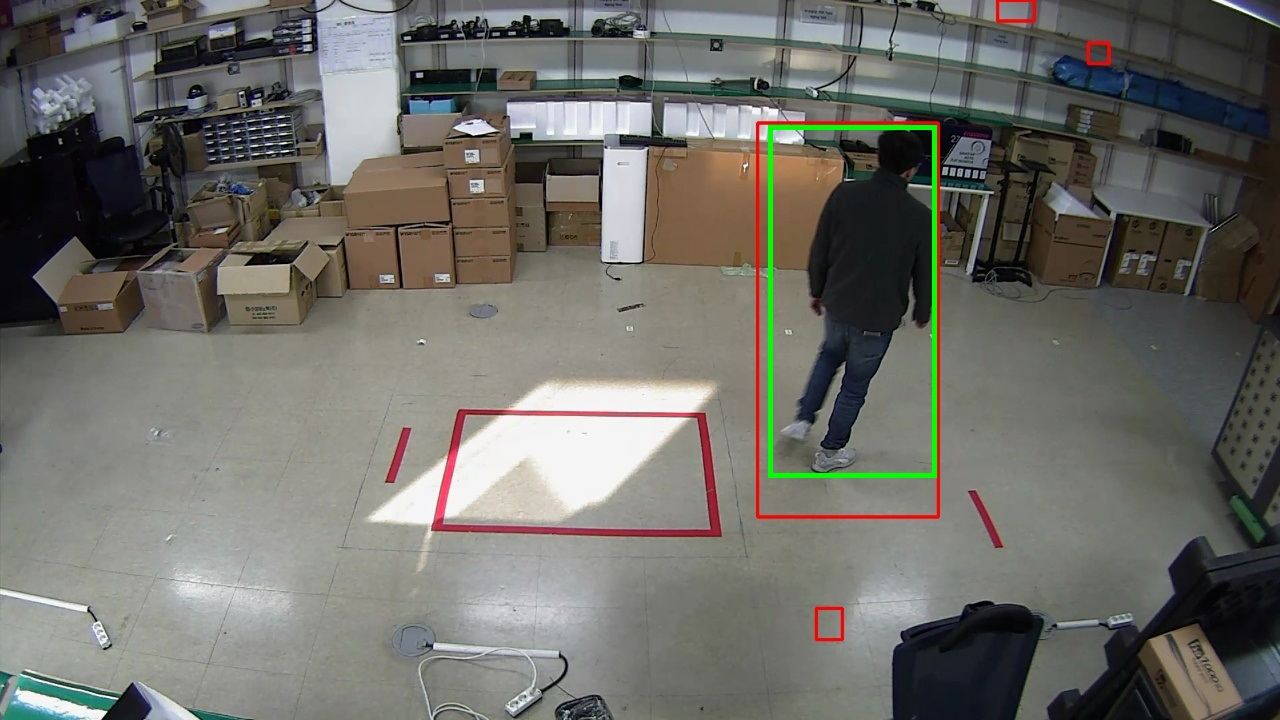
\includegraphics[width=0.25\linewidth]{Figures/1500_track.jpg}
}
\subfloat[]
{
    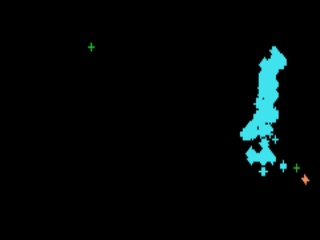
\includegraphics[scale=0.26]{Figures/1537_res.jpg}
}
\subfloat[]
{
    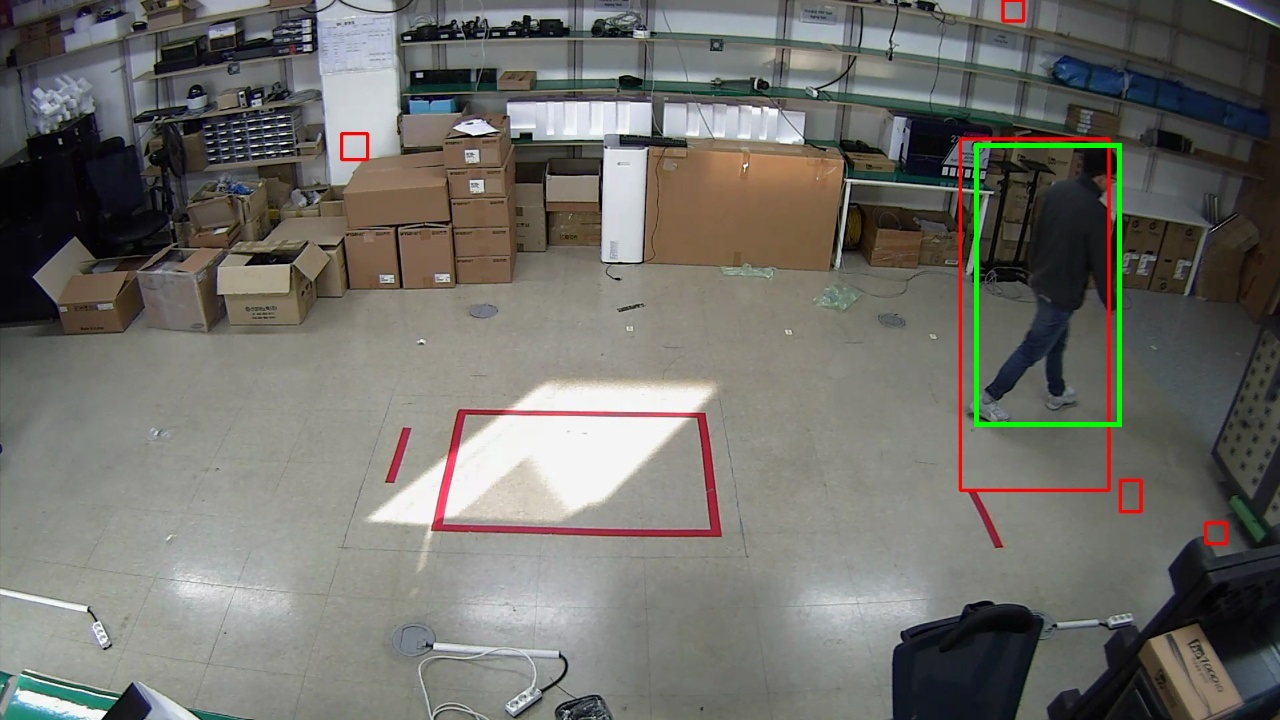
\includegraphics[width=0.25\linewidth]{Figures/1536_track.jpg}
}\\
\subfloat[]
{
    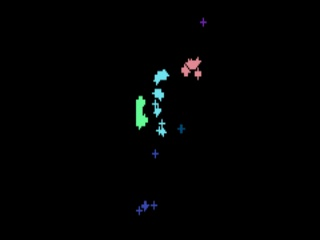
\includegraphics[scale=0.26]{Figures/3940_res.jpg}
}
\subfloat[]
{
    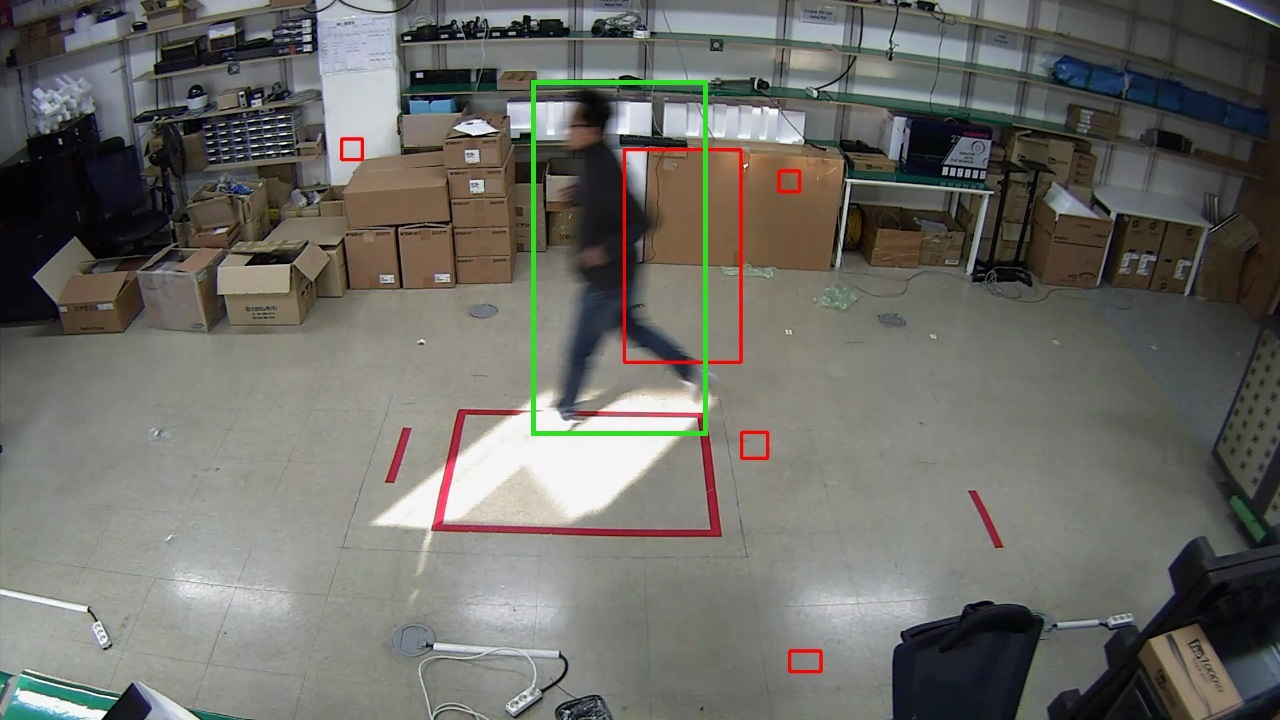
\includegraphics[width=0.25\linewidth]{Figures/3939_track.jpg}
}
\subfloat[]
{
    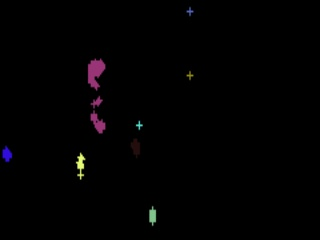
\includegraphics[scale=0.26]{Figures/3949_res.jpg}
}
\subfloat[]
{
    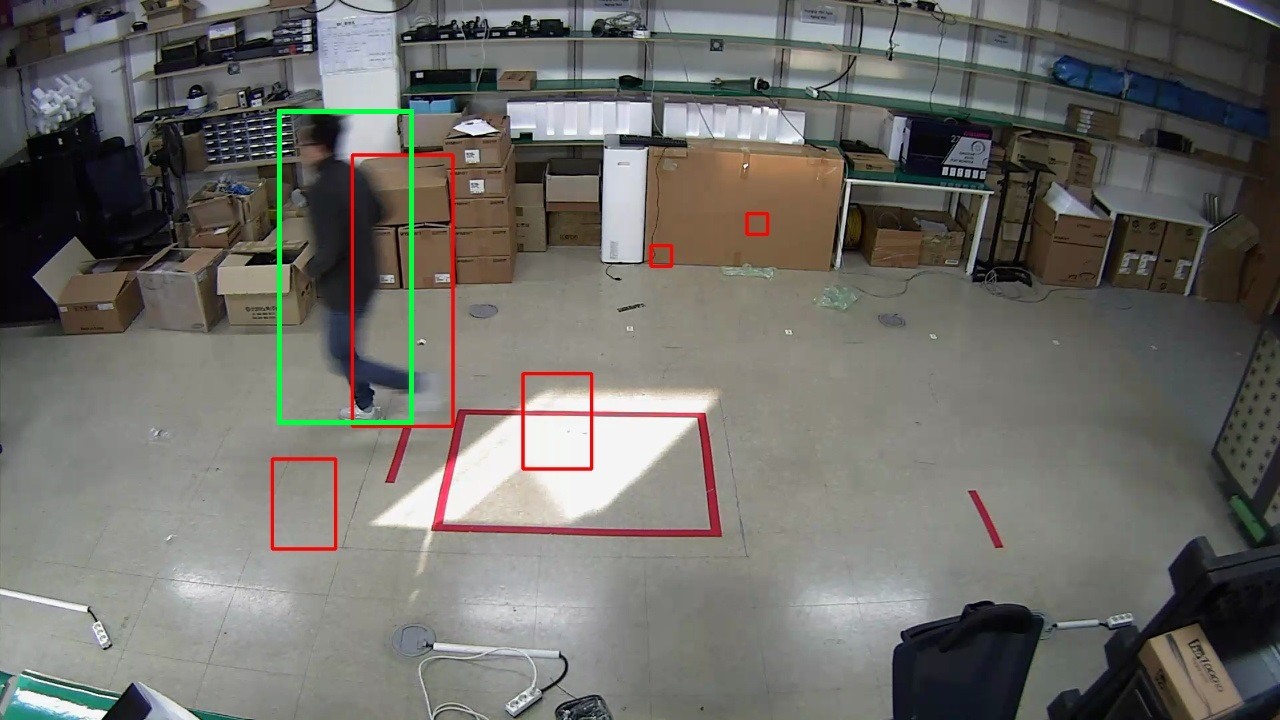
\includegraphics[width=0.25\linewidth]{Figures/3949_track.jpg}
}\\
\subfloat[]
{
    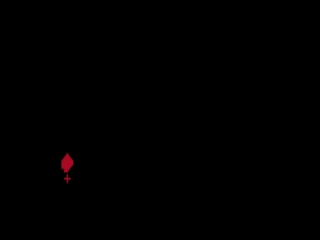
\includegraphics[scale=0.26]{Figures/370_res.jpg}
}
\subfloat[]
{
    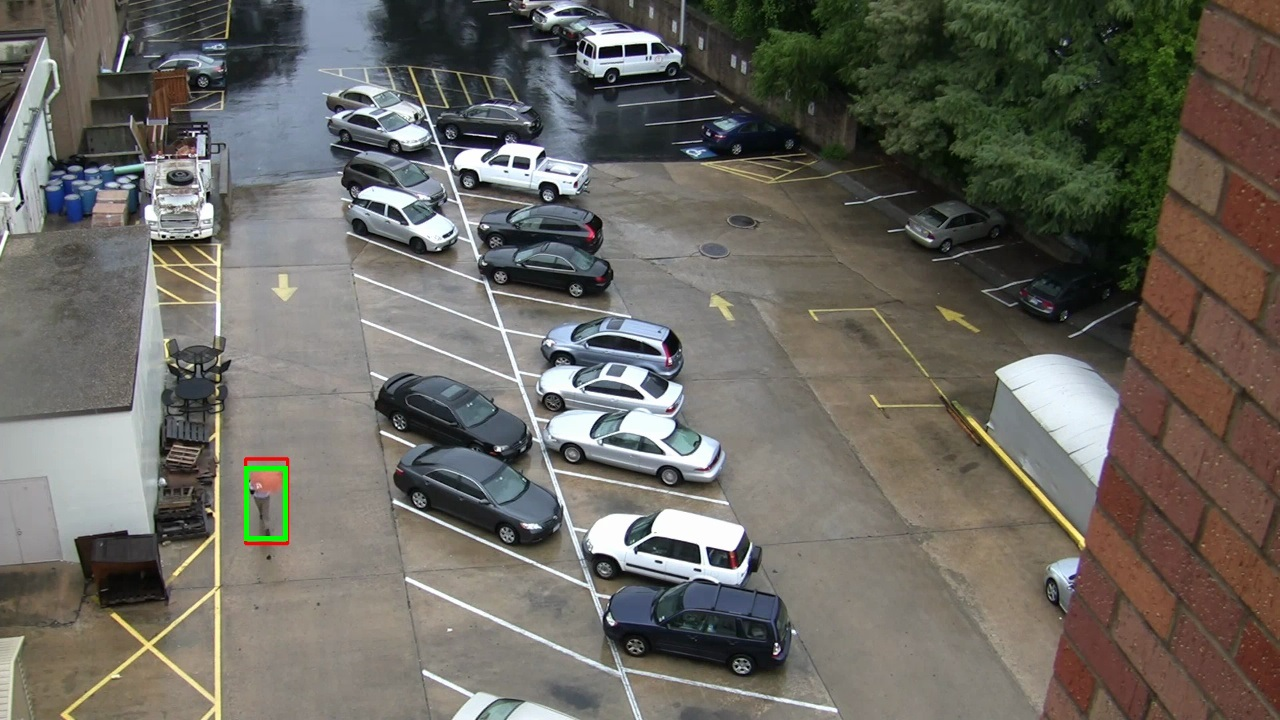
\includegraphics[width=0.25\linewidth]{Figures/370_track.jpg}
}
\subfloat[]
{
    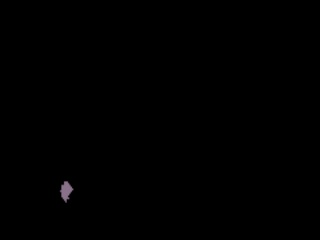
\includegraphics[scale=0.26]{Figures/435_res.jpg}
}
\subfloat[]
{
    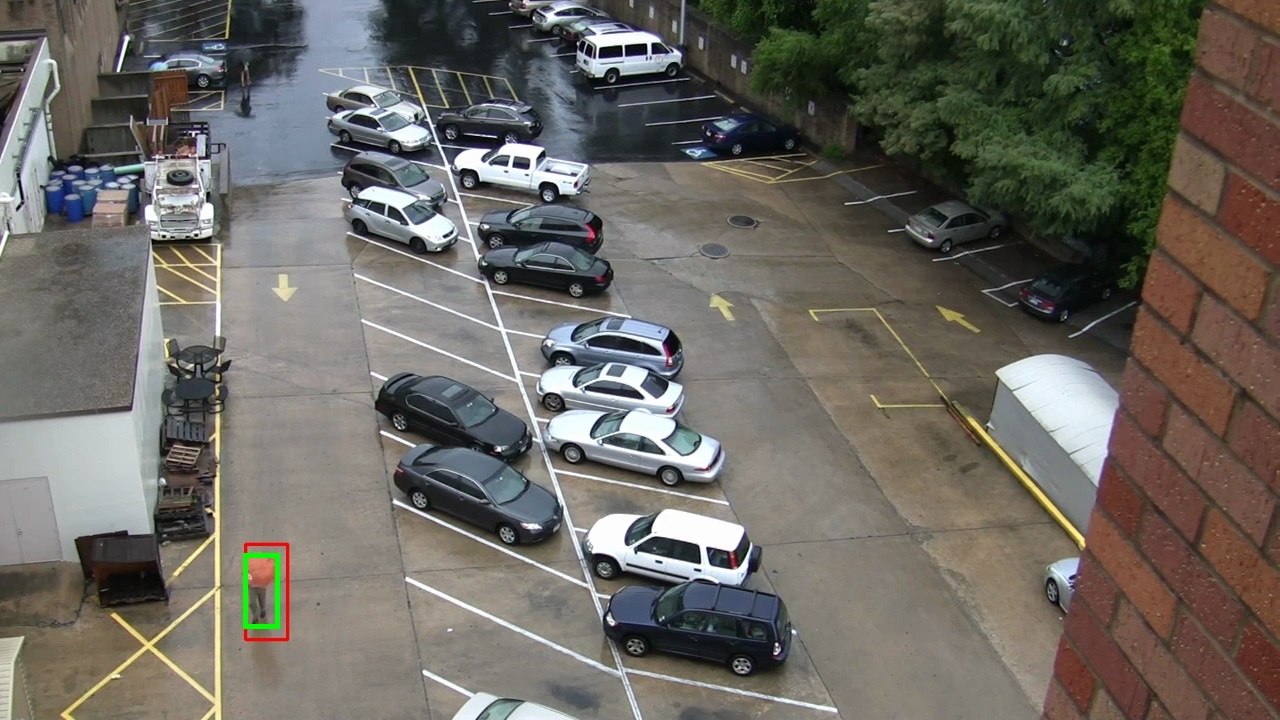
\includegraphics[width=0.25\linewidth]{Figures/435_track.jpg}
}
\caption{Moving objects detection by the proposed method in different scenarios: (a, b, c, d) human walking; (e, f, g, h) human running; (i, j, k, l) test with a far distance of camera.}
\label{fig:objectdetect}
\end{figure*}

\begin{table}[]
\centering
\caption{Average IoU of the moving object detection in compressed-domain in different scenarios.}
\label{tab:videotest}
\begin{tabular}{|c|c|c|c|}
\hline
\multirow{2}{*}{\textit{\begin{tabular}[c]{@{}c@{}}Video Test\\  Sequence\end{tabular}}} & \multicolumn{2}{c|}{\textit{Scenario}} & \multirow{2}{*}{\textit{IoU Average}} \\ \cline{2-3}
                                                                                         & Camera Position     & Moving Speed     &                                       \\ \hline
Our recorded test video                                                                                        & Near                & Normal           & 0.75                                  \\ \hline
Our recorded test video                                                                                        & Near                & Fast             & 0.26                                  \\ \hline
Video Test from VIRAT                                                                                        & Far                 & Normal           & 0.6                                   \\ \hline
\end{tabular}
\end{table}

\begin{table}[]
\centering
\caption{Average per-frame running times for preprocessing and tracking procedures. Values are expressed in miliseconds (ms) and frame per second(FPS).}
\label{tab:timemessasure}
\begin{tabular}{|c|c|c|c|}
\hline
\textit{Frame Size} & \textit{ST-MRF{[}16{]}} & \textit{Graph Cuts{[}15{]}} & \textit{Proposed Method} \\ \hline
1280x720            & 64 ms (16 FPS)         & 62 ms (17 FPS)              & \textbf{39 ms (26 FPS)}  \\ \hline
1920x1080           & N/A                    & N/A                        & \textbf{69 ms (14 FPS)}  \\ \hline
\end{tabular}
\end{table}
The green bounding boxes shown in the Figure are ground-truth bounding boxes, while the red bounding boxes are detected objects using the proposed method.The average IoU scores are shown in detail for each scenario in Table \ref{tab:videotest}. The results show that when a camera is placed at a close distance and the human does not move fast (i.e, human walking), the proposed method detected well and achieved good average IoU score of 0.75. However, when speed of human is fast in case of running or the camera is in far distance, the MV's density is decreased, the detector return lower average IoU scores. For object tracking evaluation, the scenarios are run with multiple times with different detection score threshold $\alpha$ of 0.25, 0.4 and 0.5 with the results are shown in Figure  \ref{fig:objecttracking}. 
\begin{figure*}
\centering
\subfloat[]
{
    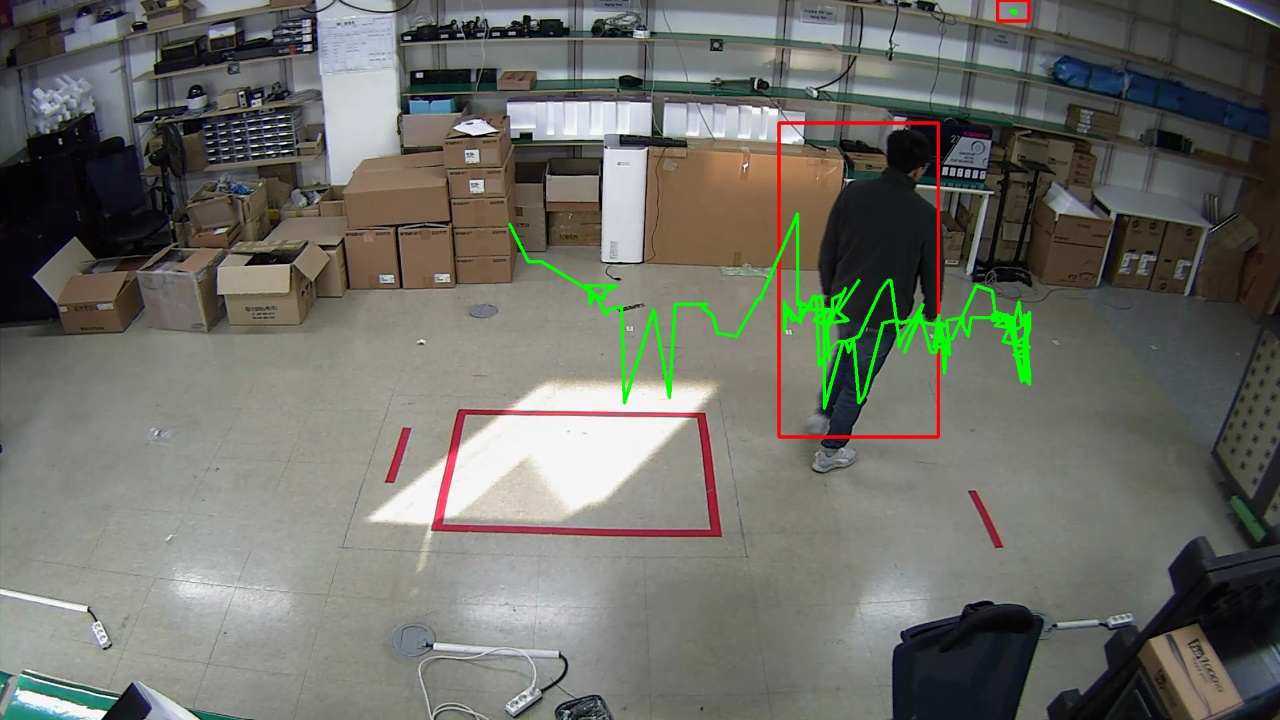
\includegraphics[width=0.3\linewidth]{Figures/1502_025.jpg}
}
\subfloat[]
{
    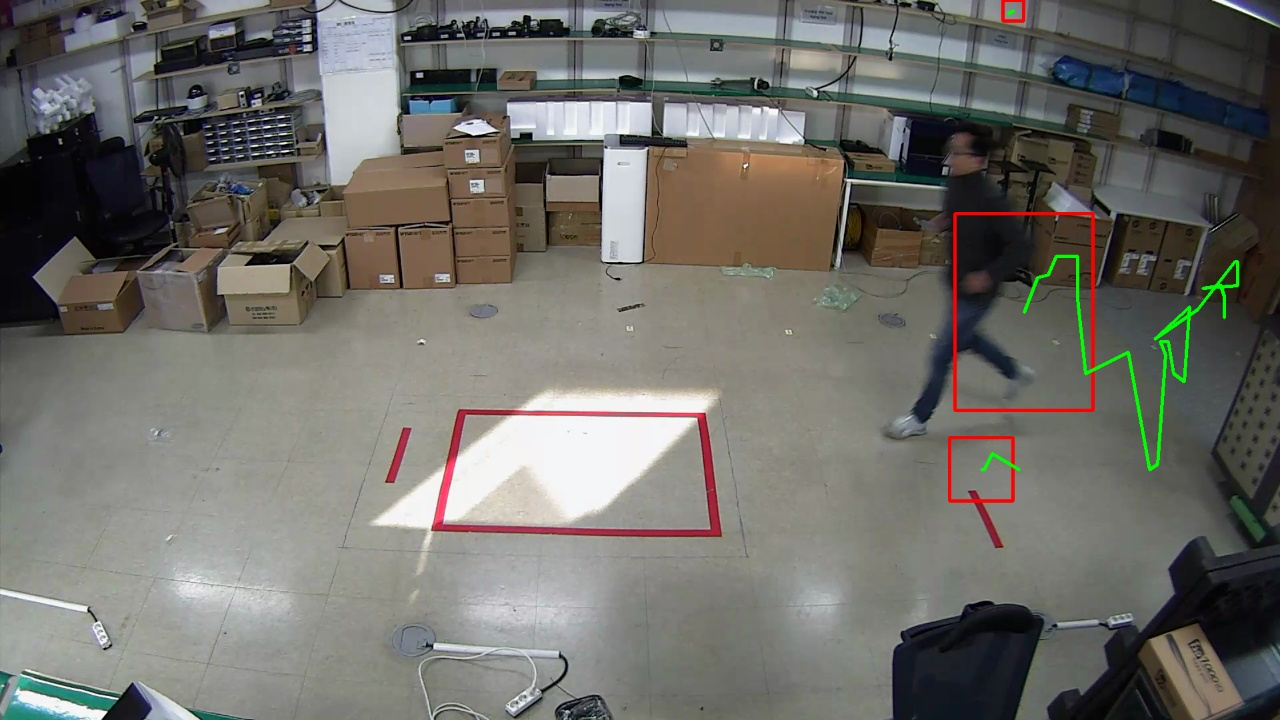
\includegraphics[width=0.3\linewidth]{Figures/3923_025.jpg}
}
\subfloat[]
{
    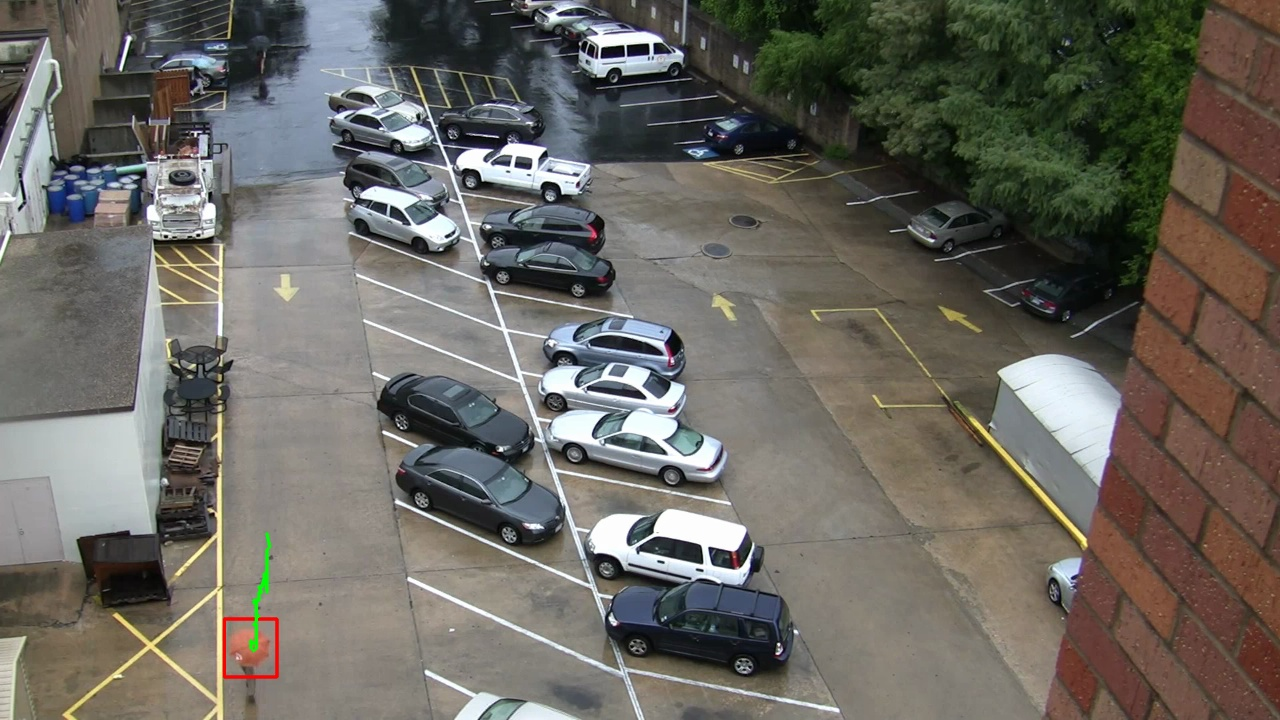
\includegraphics[width=0.3\linewidth]{Figures/478_025.jpg}
}\\
\subfloat[]
{
    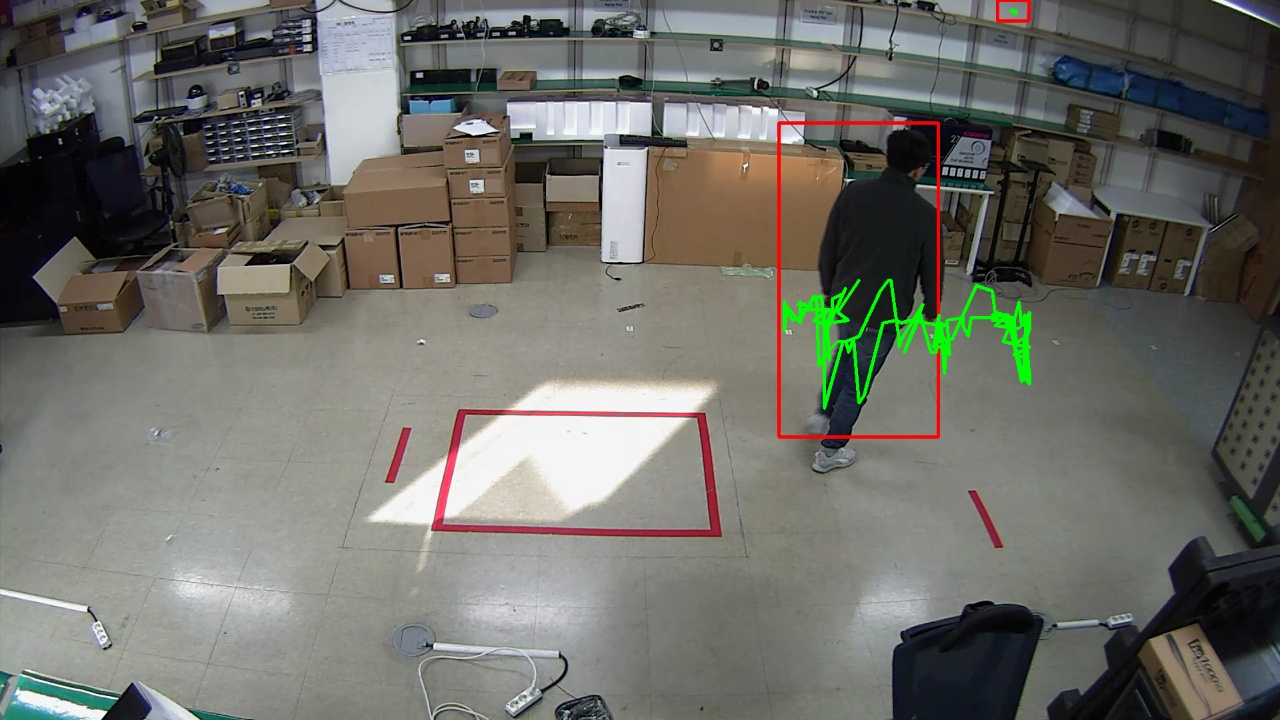
\includegraphics[width=0.3\linewidth]{Figures/1502_04.jpg}
}
\subfloat[]
{
    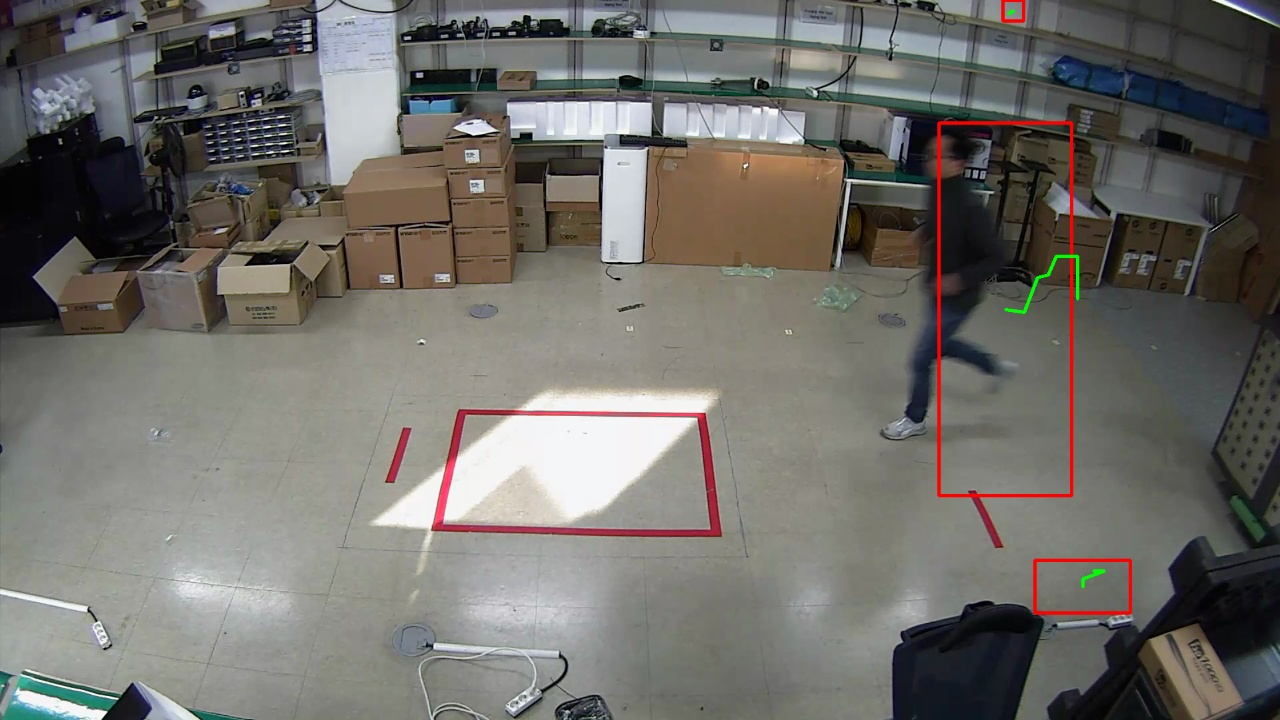
\includegraphics[width=0.3\linewidth]{Figures/3923_04.jpg}
}
\subfloat[]
{
    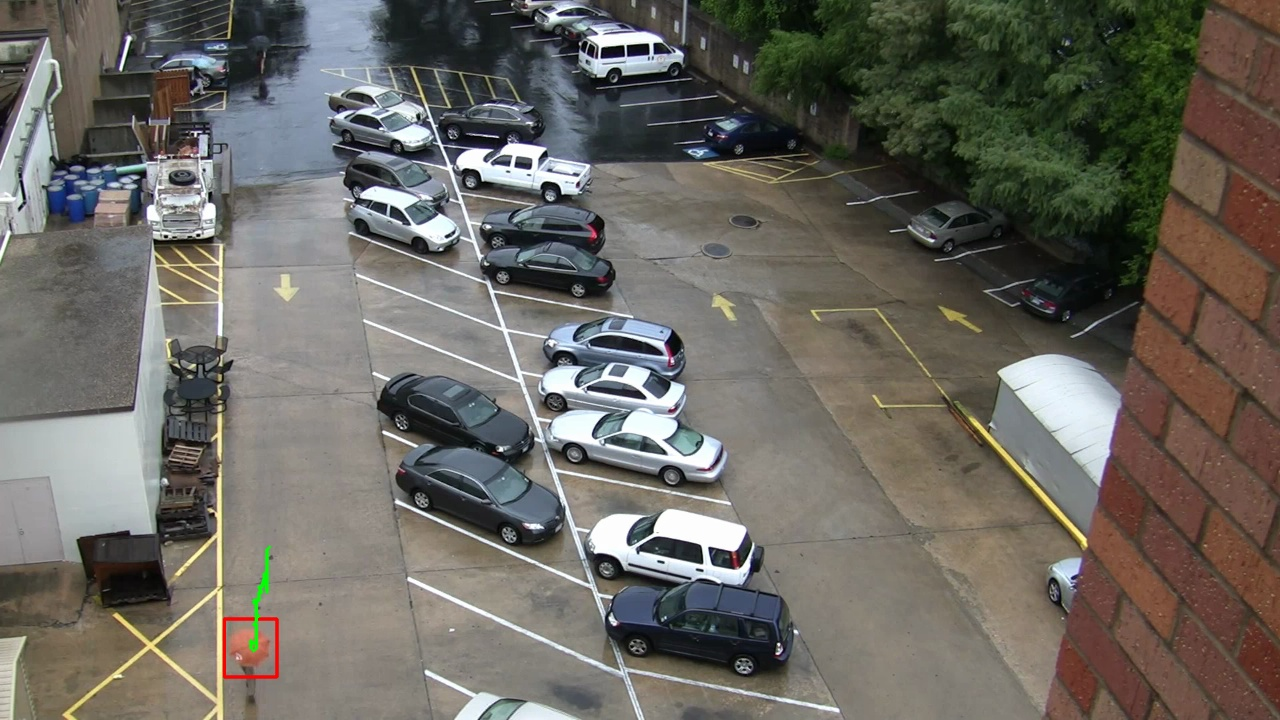
\includegraphics[width=0.3\linewidth]{Figures/478_04.jpg}
}\\
\subfloat[]
{
    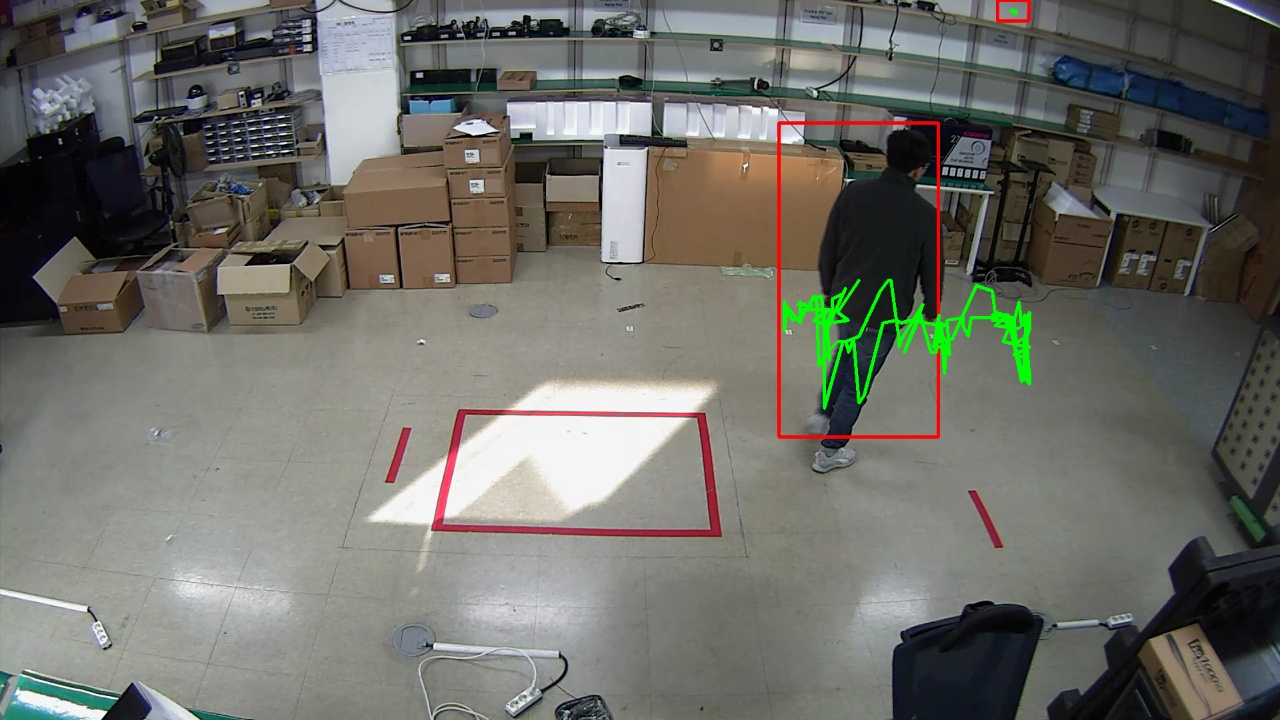
\includegraphics[width=0.3\linewidth]{Figures/1502_04.jpg}
}
\subfloat[]
{
    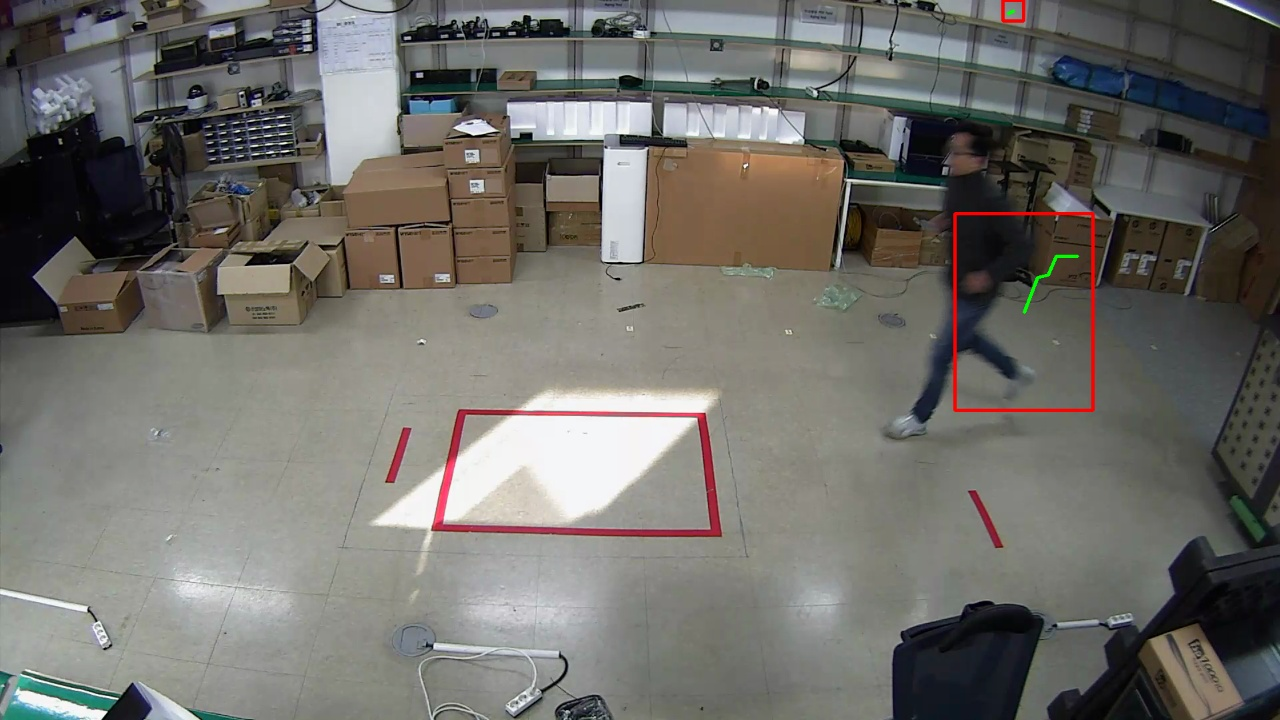
\includegraphics[width=0.3\linewidth]{Figures/3923_05.jpg}
}
\subfloat[]
{
    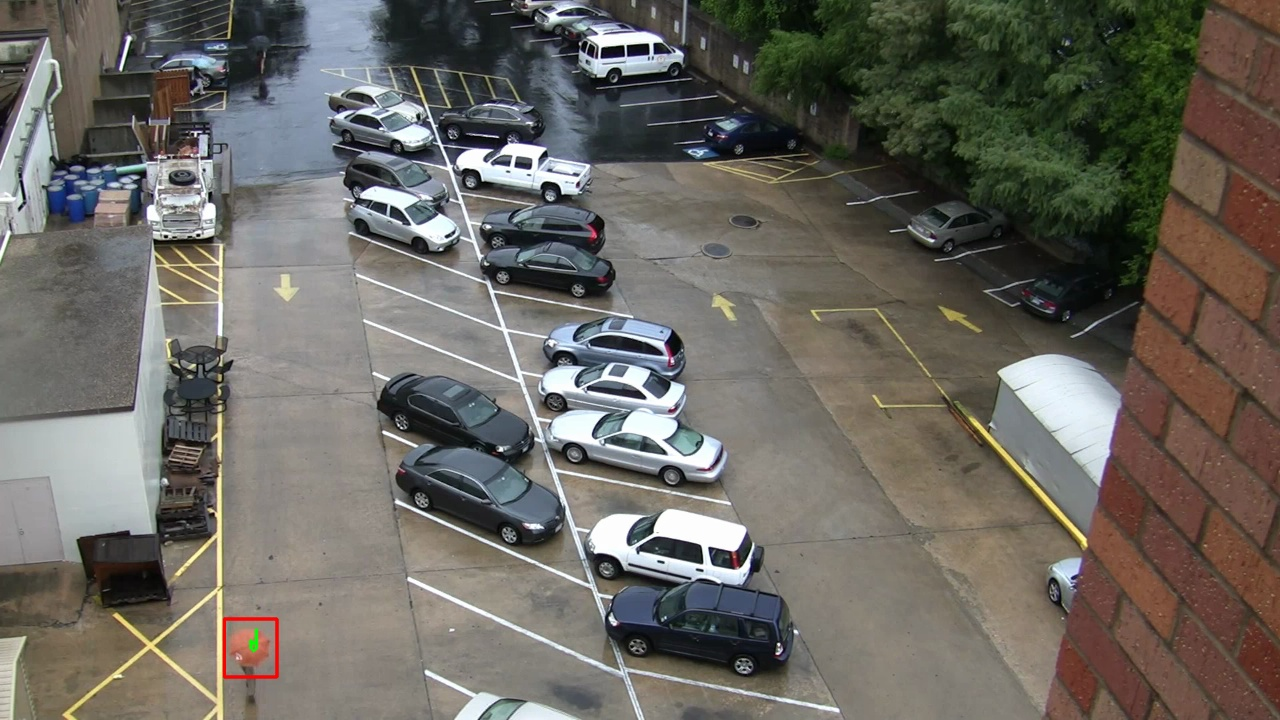
\includegraphics[width=0.3\linewidth]{Figures/478_05.jpg}
}
\caption{Moving objects tracking by the proposed method with different $\alpha$ thresholds: $\alpha$ = 0.25 in (a, b, c), $\alpha$ = 0.4 in (d, e, f) and $\alpha$ = 0.5 in (d, e, f).}
\label{fig:objecttracking}
\end{figure*}
In this experiment, each $\alpha$ threshold was applied for three same scenarios of human walking in Figure \ref{fig:objecttracking} (a, d, g), human running in Figure \ref{fig:objecttracking} (b, e, h) and the far camera distance in Figure \ref{fig:objecttracking} (c, f, i).  We see that with each test scenario, with lower $\alpha$ threshold value,the tracking object capability is better with longer the object trajactories. However, it will increase the number of false alarm detection if the noise MVs apprear frequently in some specified areas.\\ To optimize the running time speed as well as the performance, the edge node and cloud node all are implemented in C++ using the multithread architecture. We observe that the proposed method does not indicate additional computational difficulty and achieve the approved evaluated results in terms of processing time when compared with previous studies \cite{bombardelli2018efficient} \cite{khatoonabadi2012video}. The average comsuming time  is messasured with different video resolutions and shown in Table \ref{tab:timemessasure}. Compare to other studies, the average processing time for high definition resolution video is approximately 39ms/frame, which outperforms most of the state of art method. This indicates that the proposed algorithm almost handles the data in real-time. 

\section{Performance Evaluation Results}
 In this experiment, the proposed edge-to-clound platform will be implemented and evaluated. Our recored video test sequence is selected because of including different the moving object speeds. After experiments using different $\alpha$ in different scenarios, we found that the optimal $\alpha$ is 0.5 for this scenario. The entire demonstration was recorded and uploaded \cite{source}. The evaluated performances of the demonstration are presented in detail as follows.
 
 \subsection{Computing Resources Consumption}
\begin{figure*}
\centering
\subfloat[]
{
    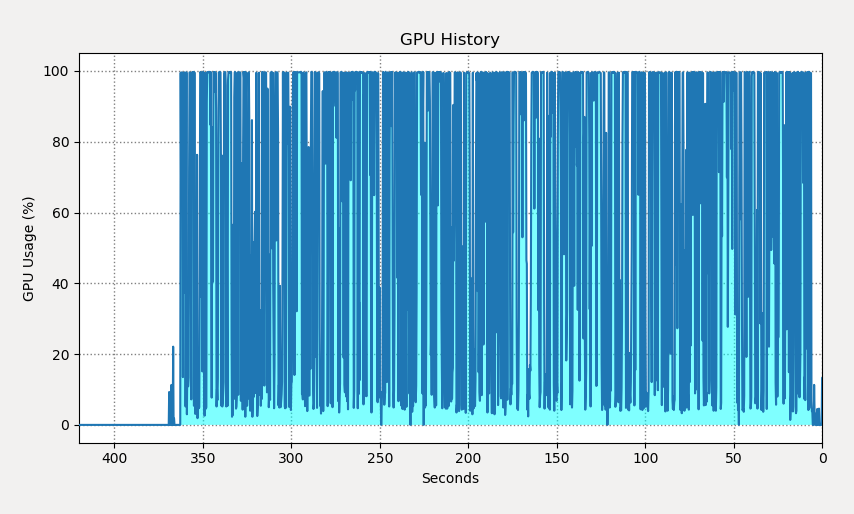
\includegraphics[scale=0.25]{Figures/gpu_c.png}
}
\subfloat[]
{
    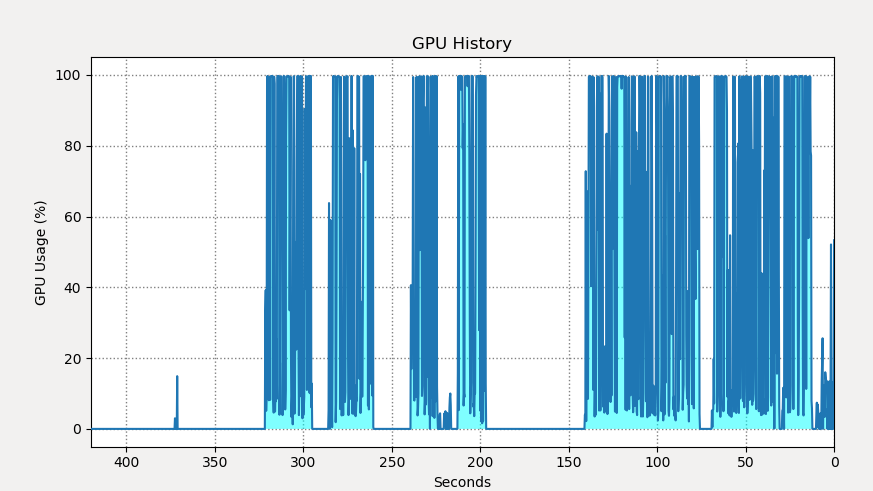
\includegraphics[scale=0.25]{Figures/gpu_p.png}
}
\caption{GPU Monitoring: (a)  With the conventional method, (b)  With the proposed method.}
\label{fig:gpu}
\end{figure*}
\begin{figure*}
\centering
\subfloat[]
{
    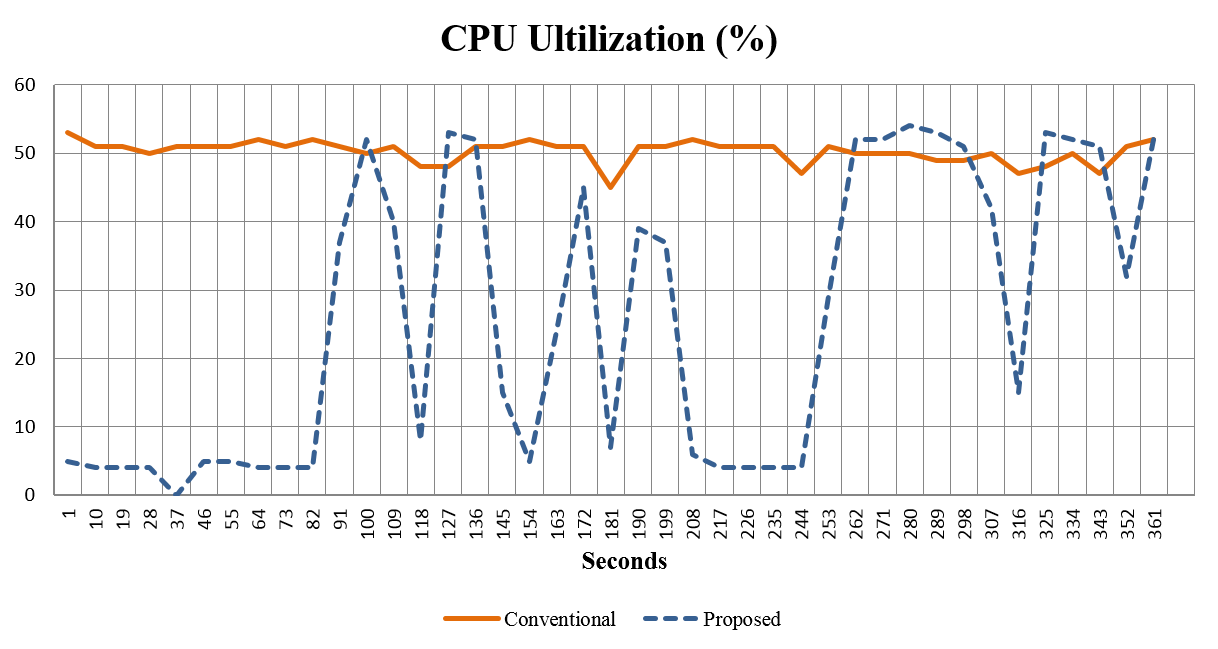
\includegraphics[scale=0.7]{Figures/cpu.png}
}
\caption{CPU Monitoring with both the conventional method and the proposed method.}
\label{fig:cpu}
\end{figure*}
\begin{figure*}
\centering
\subfloat[]
{
    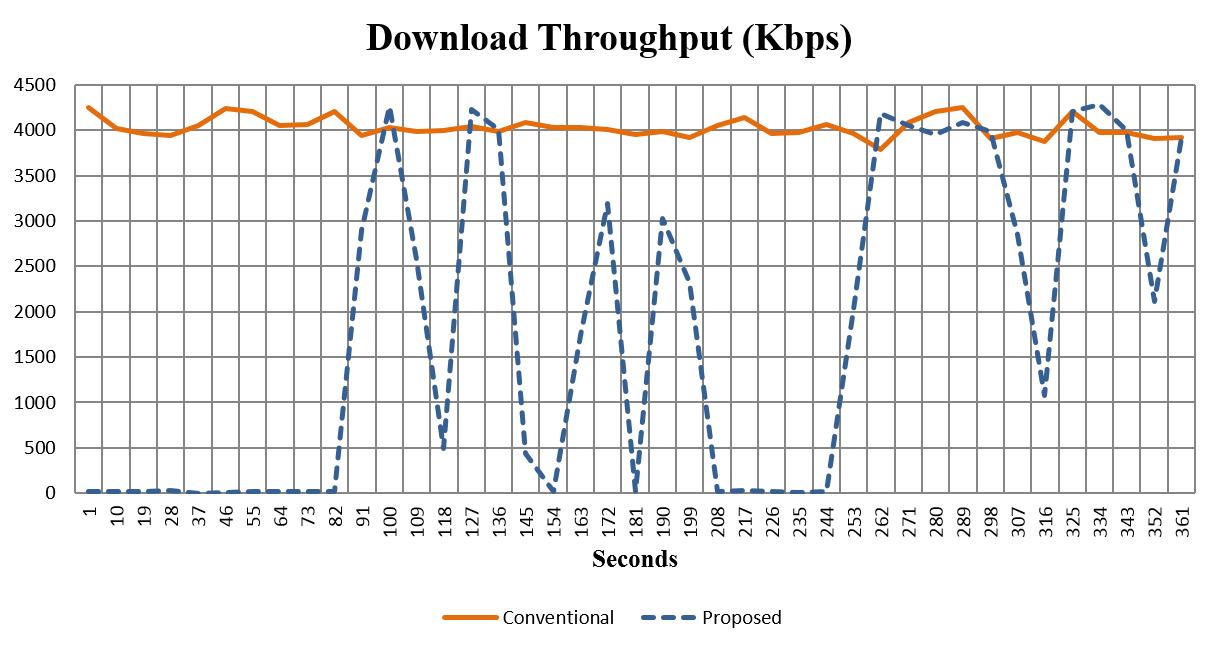
\includegraphics[scale=0.7]{Figures/network.png}
}
\caption{Network download throughput monitoring with both the conventional method and the proposed method.}
\label{fig:network}
\end{figure*}
\begin{table}[]
\centering
\caption{Average computing resources of both the conventional method and the proposed method.}
\label{tab:computingresource}
\begin{tabular}{|c|c|c|c|}
\hline
\textbf{Computing Resources}                                         & \textbf{Conventional Method} & \textbf{Proposed Method} & \textbf{Performance Ratio} \\ \hline
GPU Utilization (\%)                                                  & 65.61                        & 33.73                    & 0.51                       \\ \hline
CPU Utilization (\%)                                                  & 50.24                        & 25.9                     & 0.51                       \\ \hline
\begin{tabular}[c]{@{}c@{}}Download Throughput\\ (Kbps)\end{tabular} & 4028                         & 1808.2                   & 0.45                       \\ \hline
\end{tabular}
\end{table}
During demonstration of  intrusion detection application, the clouds node’s computing resources, including CPU, GPU utilization, and network download throughput, was monitored and recorded and shown in Figure \ref{fig:sysdesign}. For comparison, the performance results are compared to that of the conventional method, which did not use edge node as shown in Figure \ref{fig:overall}. The results indicate that both methods achieve the same accuracy in terms of alert notification when humans entered the restricted area. The demonstration's record of both these methods are uploaded to \cite{convential}, \cite{proposed}. In terms of consumption of computational resources, GPU, CPU utilizations, and download throughput of both methods are measured and presented in Figure \ref{fig:gpu}, \ref{fig:cpu} and \ref{fig:network} respectively. The figures clearly show the advantage of using the proposed method. While the conventional method of processing all video frames captured from camera leads to consumption of computational resources, our method only processes when there is motion, and therefore computational resources are dynamically allocated and economical. Another observation is that our proposed method is extremely effective for detecting motion of the scene compared to the ground-truth motion time in Table \ref{tab:motiontime}. In detail,  the time for consuming and releasing computing resources of VA server was matched with the time for appearance and disappearance of motion in ground-truth table. Since the conventional method processes all video frames, we assume that the its computing resource average is S. According to formulation \ref{eqn:5}, the performance ratio of both methods in this video will be as follows:\\
\begin{equation}
\label{eqn:10}
\frac{Comp_{p}}{Comp_{c}}=\frac{(K*S+(N-K)*T)}{N*S}=\frac{K}{N} + (1 - \frac{K}{N})*\frac{T}{S}=\frac{140}{360} + (1 - \frac{140}{360})*\frac{T}{S} = 0.4 + 0.6*\frac{T}{S}
\end{equation}
Compared with the performance ratio, which is calculated in real scenario test in Table \ref{tab:computingresource}, our performance theory model and real measurement are matching and reasonable.